\chapter{Implementando Laboratório Virtual}\label{cap:proposta}

O presente projeto propõe o desenvolvimento de um laboratório virtual como de ambiente para o ensino de modelagem e controle de CubeSats por meio de simulação. Utilizando ferramentas aberta e livres contornando o problema de custo. E de roteiros para instalação, configuração e uso, contornando o problema da curva de aprendizado.

\section{Requisitos}\label{Requisitos}

Para a realização do presente projeto está foi escolhido as aplicações a seguir:

\begin{itemize}
    \item Ubuntu 24.04 LTS
    \item JSBSim
    \item FlightGear
    \item Python
    \item Blender
\end{itemize}

O JSBSim é uma plataforma de código aberto para modelagem de dinâmica de voo, simulando a física e a matemática dos 6 graus de liberdade do movimento de aeronaves, foguetes e outros veículos aéreos. Ela pode ser executada independentemente ou integrada a outros simuladores como o FlightGear, \citeonline{manualJSBSim}.

O FlightGear por sua vez é um simulador de voo gratuito e de código aberto que oferece uma experiência realista de voo para várias plataformas incluindo o Windows, macOS e Linux podendo ser usado para pesquisa. Quando integrado ao JSBSim ele oferece uma interface visual, permitindo visualizar o comportamento de uma aeronave simuladas, \citeonline{manualFlightGear}.

Ambos programas são escritos em C++, mas possuem integração com o Python, os modelos das aeronaves são descritos em XML, onde é incluído propriedades inerciais, modelos aerodinâmicos, sistema e componentes.

Para o funcionamento é previsto o hardware mínimo a seguir:

\begin{itemize}
    \item Memória: 4 GB
    \item Disco: SSD 120 GB
    \item Placa de Vídeo: 1GB Dedicada
    \item Processador: QuadCore 2.1 GHz
\end{itemize}

É possível encontrar em suas respectivas páginas oficiais de forma, o sistema operacional Ubuntu, o modelo de dinâmica de voo JSBSim e o simulador de voo FlightGear.

\section{CubeSat Design}

Define-se o cubesat como um corpo rígido homogêneo, o mesmo 10 cm de comprimento, 20 cm de lagura e 30 cm de altura e 5kg de massa.

Considerando que o eixo do corpo está alinhado com os eixos principais de Inércia, tem-se:

\begin{verbatim}
<mass_balance>
	<ixx unit="KG*M2"> 0.05416667 </ixx>
	<iyy unit="KG*M2"> 0.04166667 </iyy>
	<izz unit="KG*M2"> 0.02083333 </izz>
	<ixy unit="KG*M2"> 0 </ixy>
	<ixz unit="KG*M2"> 0 </ixz>
	<iyz unit="KG*M2"> 0 </iyz>
	<emptywt unit="KG"> 5 </emptywt>
	<location name="CG" unit="M">
		<x> 0 </x>
		<y> 0 </y>
		<z> 0 </z>
	</location>
</mass_balance>

\end{verbatim}

Define-se a roda de reação como um corpo rígido homogêneo cilíndrico, de raio 0.0435 m e massa de 0.137kg.

Considerando que o eixo do corpo está alinhado com os eixos principais de Inércia, tem-se:

\begin{verbatim}
<!-- ROTATION IN X -->
	<force name="RDR_x_1" frame="BODY">
	<function>
		<property> actuator/RDR-x </property>
	</function>
	<location unit="M">
		<x>0</x>
		<y>0</y>
		<z>0.5</z>
	</location>
	<direction>
		<x>  0 </x>
		<y>  1 </y>
		<z>  0 </z>
	</direction>
</force>

<force name="RDR_x_2" frame="BODY">
	<function>
		<property> actuator/RDR-x </property>
	</function>
	<location unit="M">
		<x>0</x>
		<y>0</y>
		<z>-0.5</z>
	</location>
	<direction>
		<x>  0 </x>
		<y> -1 </y>
		<z>  0 </z>
	</direction>
</force>
\end{verbatim}

Perceba que para caracterização devida do momento é feita um binário de força.

\section{Control Design}

foi escolhido os seguites polos 
[-8.08825423e-05+0.j   -6.93278934e-05+0.j   -7.51052178e-05-0.01j
-7.51052178e-05+0.01j]

por serem entre 6 a 7 vezes mais lento que 1.15546489e-05 que é o polo da roda de reação

A matriz de ganhos ficou 

\begin{equation}
	K = \begin{bmatrix}
		-6.13702972 \times 10^{-4} & 6.00828148 \times 10^{-4} & -6.08004453 \times 10^{0} & 7.70729819 \times 10^{0} \\
		-1.98023000 \times 10^{-4} & 3.06189753 \times 10^{-4} & -2.54675474 \times 10^{2} & 2.38676450 \times 10^{0}
	\end{bmatrix}
\end{equation}

\begin{figure}[htpb]
	\centering
	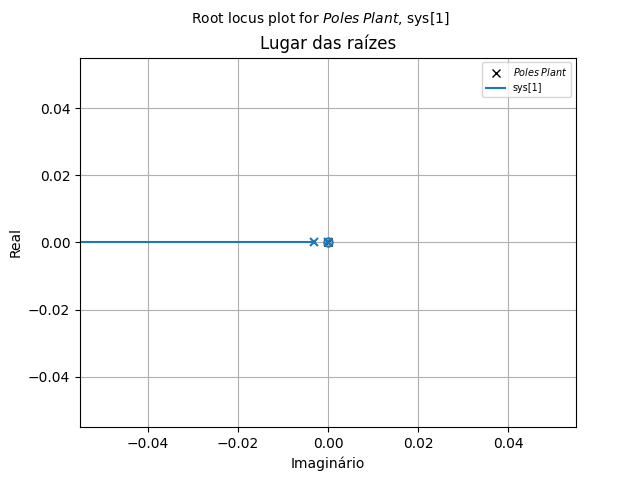
\includegraphics[scale0.751]{figs/resultado_lugar_das_raizes.png}
	\caption{Lugar das Raízes}
	\label{fig:15}
\end{figure}

\begin{figure}[htpb]
	\centering
	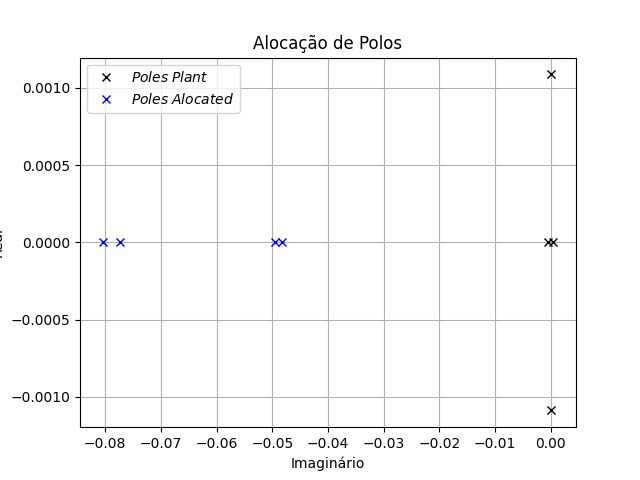
\includegraphics[scale0.5]{figs/resultado_alocacao_polos.png}
	\caption{Alocação de polos}
	\label{fig:15}
\end{figure}


\begin{figure}[htpb]
	\centering
	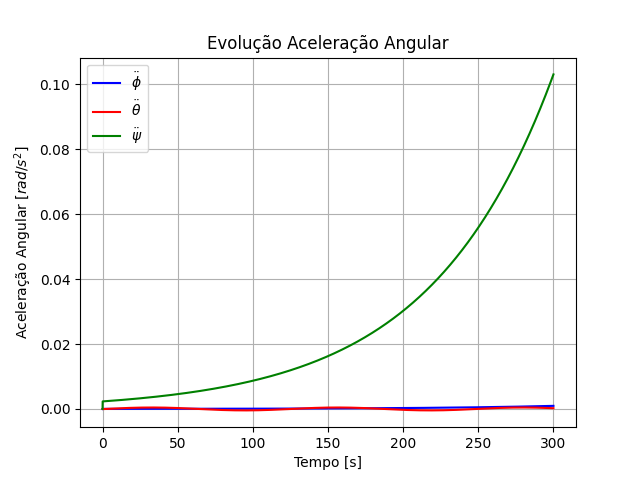
\includegraphics[scale=1]{figs/resultado_evolucao_acelang_linear.png}
	\caption{Resultado Aceleração Angular Controle Planta Linearizada}
	\label{fig:15}
\end{figure}

\begin{figure}[htpb]
	\centering
	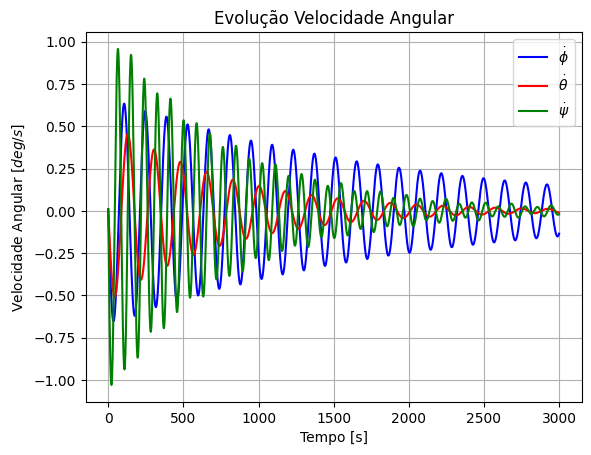
\includegraphics[scale=1]{figs/resultado_evolucao_velang_linear.png}
	\caption{Resultado Velocidade Angular Controle Planta Linearizada}
\label{fig:15}
\end{figure}

\begin{figure}[htpb]
	\centering
	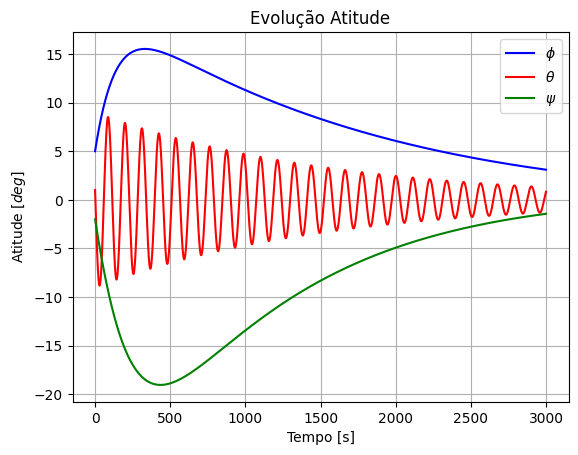
\includegraphics[scale=1]{figs/resultado_evolucao_atitude_linear.png}
	\caption{Resultado Atitude Controle Planta Linearizada}
	\label{fig:15}
\end{figure}


\section{Simulação Dinâmica}

r_SCGI = np.array([2.25526213722520e+006, -3.00492371279401e+006, -5.84397331427593e+006]) # m
v_SCGI = np.array([-5.19923341417592e+003, 3.82519438208177e+003, -3.97333292224794e+003]) # m/s


\begin{figure}[htpb]
	\centering
	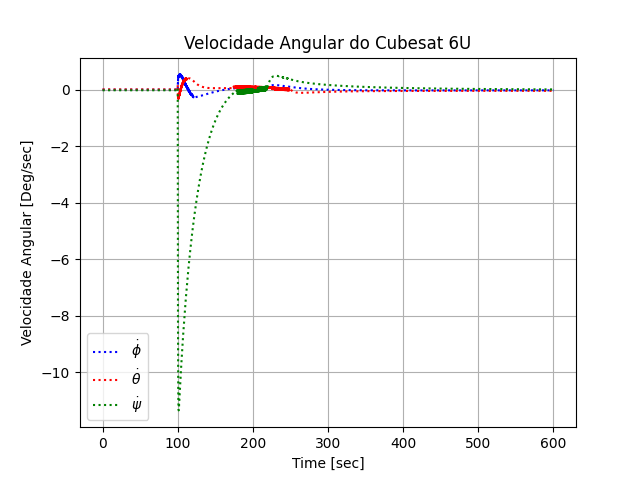
\includegraphics[scale=1]{figs/resultado_simulacao_dinamica_velocidade.png}
	\caption{Resultado Atitude Simulação}
	\label{fig:15}
\end{figure}

\begin{figure}[htpb]
	\centering
	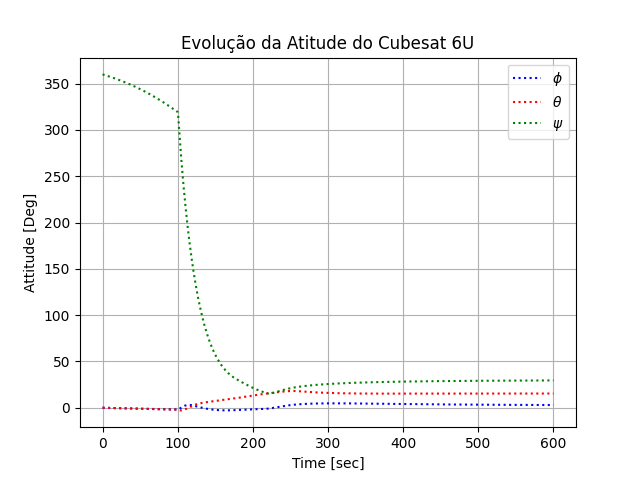
\includegraphics[scale=1]{figs/resultado_simulacao_dinamica_atitude.png}
	\caption{Resultado Velocidade Simulação}
	\label{fig:15}
\end{figure}

\section{Considerações Finais}




